\chapter{SCOBY Machine \& Materials}


\section{Overview}

In the same way as for the environent control project with the scoby, we had to think about how machines can help us make this new material our own, in much the same way as 3D printers popularized the use of PLA. 

The methods and machines presented here are designed to facilitate the use of this biomaterial, with the aim of optimizing the production of bacterial cellulose and changing the growing conditions to produce 3D cellulose. 

In addition, unlike mycelium, which unfolds in a substrate contained in a mold, cellulose requires more attention to shape channelling, both for molding and demolding. 

\begin{figure}[h]
    \centering
    \includegraphics{images/IMG_4126.jpg}
    \caption{Bacterial cellulose at the sufface and it meidium}
    \label{fig:}
\end{figure} 

\section{Systems design}


In the traditional approach, cellulose grows on the surface of the liquid, which means that the cellulose takes on a flat shape \- the shape of the container in which the bacterial cellulose grows. 

With the bioreactor, there are two objectives. on the one hand, to optimize production. On the other hand, to modify the natural growth of poccesus in order to be able to make more complex shapes than 2D shapes. 

To achieve this, the method used is to introduce a 3D shape that rotates on the surface of the liquid so that the cellulose can adhere to the shape and push against it. As shown in the following diagram. 

the bioreactor incorporates a rotating framework, typically shaped to encourage cellulose attachment and buildup in desired forms beyond a simple flat surface. This framework is submerged in a controlled culture medium, allowing the bacteria to deposit cellulose around a defined 3D scaffold as it rotates. The rotation ensures even cellulose distribution, encouraging layers to adhere around the object and gradually form into three-dimensional shapes.
\begin{figure}[h]
    \centering
    \includegraphics{images/shema3Dscoby.png}
    \caption{System design representation for 3D bacterial cellulose}
    \label{fig:diagBC3D}
\end{figure} 

The bioreactor takes the form of a closed space like a box, with openings covered with microporous plaster to allow air to pass through without contaminating the space. Into which the culture medium can be introduced.
It is generally located in a closed space in which a heating mat is installed to maintain a suitable temperature for better cellulose development. 
heating mat helps sustain an optimal temperature for bacterial activity, while microporous openings enable airflow, preventing contamination while ensuring that the bacteria have sufficient oxygen. Adjusting rotation speed and environmental factors enables control over cellulose thickness.


\section{Manufacturing Processes \& Grow Theory}


\begin{figure}[h]
    \centering
    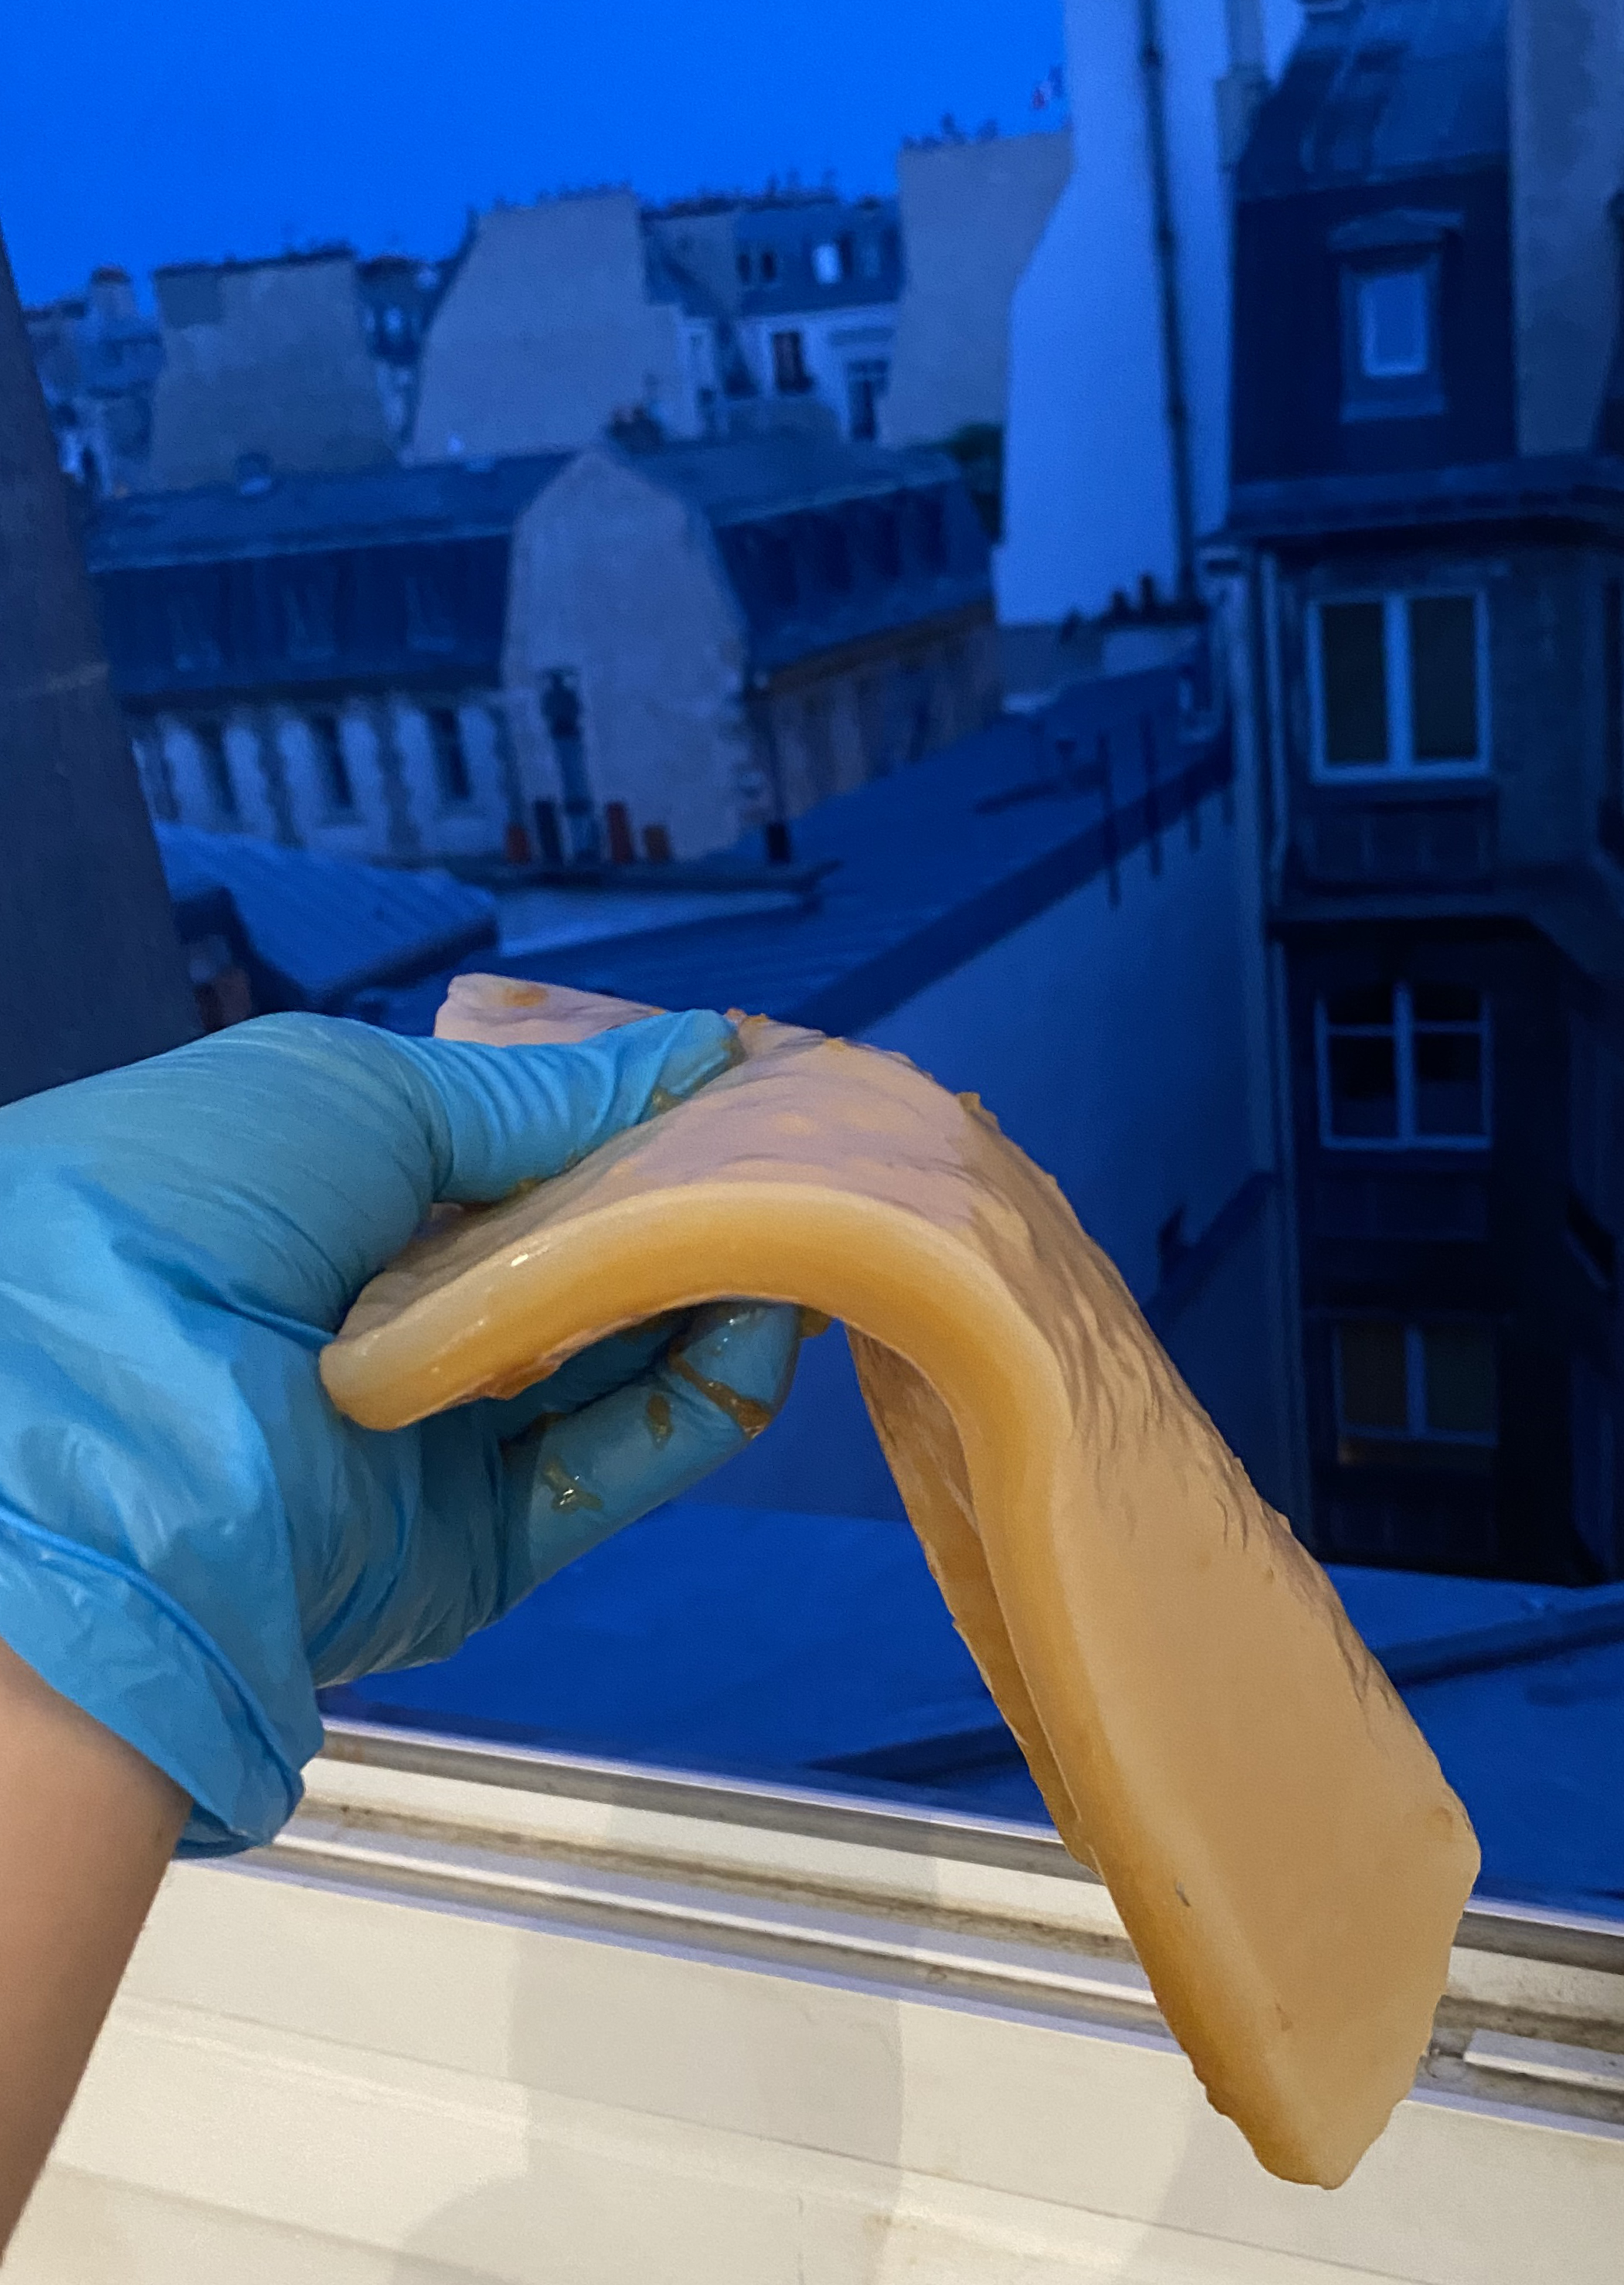
\includegraphics[width=0.7\textwidth]{images/prodperso.png}
    \caption{Bacterial cellulose after growth period}
    \label{fig:manufactureperso}
\end{figure} 

In kombucha production, bacterial cellulose naturally forms a film on the surface of the liquid medium. The Acetobacter bacteria in the SCOBY (Symbiotic Culture of Bacteria and Yeast) convert sugars in the medium into long cellulose fibers when exposed to oxygen. This fibrous structure gradually accumulates, forming a thick cellulose layer that acts as a barrier, potentially preventing other microorganisms from entering the medium. The cellulose matrix produced this way is thought to provide protection for the bacteria by limiting microbial competition.

This cellulose production process operates from the top of the solution downward. As cellulose accumulates, the older layers sink, leaving the most recently formed cellulose on the top surface exposed to oxygen. This layered formation is key to producing thick, multi-layered sheets of cellulose that can later be harvested.

The process of creating bacterial cellulose involves two main stages: preparing the culture medium and setting up the bioreactor. In preparing a homemade culture medium, freshly crushed bacterial cellulose is added to a nutrient solution composed of tea, water, sugar, and a small amount of vinegar to maintain an acidic environment conducive to bacterial growth.

\-- Boil the Water: This step sterilizes the water and allows the tea to fully infuse.

\-- Add Tea, Sugar, and Vinegar: These elements provide essential nutrients. The tea provides nitrogen, while sugar is the primary energy source for the bacteria. Vinegar lowers the pH, creating a favorable acidic environment.

\-- Cool the Solution: Allow the mixture to cool below 30°C to avoid harming the living cultures.

\-- Introduce Crushed Cellulose: Adding bacterial cellulose from an older culture introduces live bacterial strains to kickstart the cellulose production.

\begin{figure}[h]
    \centering
    \includegraphics[width=0.7\textwidth]{images/preparation.png}
    \caption{preparation of medium}
    \label{fig:manufactureperso2}
\end{figure} 
Once the medium is prepared, it is transferred into a bioreactor, typically a container that promotes even growth. After approximately 14 days, a cellulose mat forms on the surface. This mat is then harvested, and the process can be repeated to cultivate a cellulose strain optimized for desired growth characteristics.

\begin{figure}[h]
    \centering
    \includegraphics[width=0.7\textwidth]{images/IMG_4565.jpg}
    \caption{preparation of cellulose before drying process}
    \label{fig:manufactureperso3c}
\end{figure} 
Drying and Final Processing: After growth, the cellulose mat is carefully removed and dried to achieve its final texture and strength. The drying process removes about 90\% of its water content, reducing the cellulose sheet to its final shape and thickness, making it durable and ready for various applications.



\begin{figure}[h]
    \centering
    \includegraphics[width=1.2\textwidth]{images/SCOBY_diag.png}
    \caption{Classical manufacturing processes}
    \label{fig:manufacture}
\end{figure} 

\section{Contribution}

\subsection{Rotary Bioreactor}
The project consists of a rather unusual bioreactor and traditional bacterial cellulose production. The bioreactor is made up of two closed enclosures, one inside the other.

In the larger of the two, there's a heating mat to raise the temperature for faster cellulose development, and a motor with a transmission system that turns a shaft in the smaller chamber. It's in the smaller one that the growing medium will be located.

In this configuration, the cellulose will not grow on the surface but on the shape in question, which will form cellulose in 3 dimensions with the shape of the surface of the shape on the axis. 

This innovative bioreactor configuration is designed to overcome the traditional limitations of bacterial cellulose growth, which typically forms flat sheets on the surface of the liquid medium. By introducing a rotating axis and shaping system, this bioreactor enables the cultivation of cellulose in three dimensions, opening the door to new applications and geometries.

The smaller, internal chamber serves as the primary growth environment. Here, the shape to be coated in cellulose is mounted onto the rotating shaft, allowing it to continually move through the culture medium. This rotation ensures even exposure of the shape to the bacteria and nutrients, promoting uniform cellulose deposition across its surface. The movement also helps disrupt stagnation zones, improving nutrient distribution and oxygen exposure to support optimal bacterial activity.

The larger, external chamber acts as a controlled environment for the process. The heating mat is essential for maintaining an ideal temperature, typically around 25–30°C, which accelerates bacterial cellulose synthesis without compromising quality. The bioreactor's design also incorporates ventilation with microporous filters to allow oxygen exchange while preventing contamination. This ensures the bacterial culture remains healthy and active throughout the production cycle.

This method allows for precise control over the final product's geometry, enabling the creation of hollow structures, complex curves, and other intricate forms not possible with traditional surface-grown cellulose. 
\begin{figure}[h]
    \centering
    \includegraphics{images/insiderotary.png}
    \caption{Inside grow culture medium on rotary bioreactor}
    \label{fig:rotary inside}
\end{figure} 

\section{Result}

\subsection{traditional approach}


\begin{marginfigure}
    \centering
    \includegraphics{images/kombujolie.JPG}
    \caption{Bacterial cellulose (with flys inside due to contamination)}
    \label{fig:fogger}
\end{marginfigure}

With a traditional approach, as described above, the growing time is around 14 days. with scoby leather, several alternative uses are possible. however, without prior treatment, the cellulose remains impermeable. when it dries, the bacterial cellulose loses 90\% of its volume. Once dry, it can also recapture water/moisture, which can also be an interesting property, especially in medical applications.   

One of the problems that can occur during growth is that case forms between the surface of the liquid and the cellulose, resulting in strata in the bacterial cell or poor-quality cellulose. 
\begin{figure}[h]
    \centering
    \includegraphics{images/IMG_3944.jpg}
    \caption{Example of poor-quality cellulose on the bottom and good cellulose on the front (after growth). }
    \label{fig:rotary inside}
\end{figure} 

\begin{figure}[h]
    \centering
    \includegraphics{images/IMG_4567.jpg}
    \caption{different bacterial cellulose produced}
    \label{fig:rotary inside}
\end{figure} 

\subsection{rotary approach}


\begin{figure}[h]
    \centering
    \includegraphics{images/IMG_2419.jpg}
    \caption{Bacterial cellulose produced with rotary bioreactor drying}
    \label{fig:rotary inside}
\end{figure} 

The rotary bioreactor offers a significant advancement in bacterial cellulose production, particularly when aiming for three-dimensional forms. In this approach, the rotation of the mould in the culture medium accelerates cellulose deposition. This occurs because the rotation ensures continuous contact between the bacterial culture and the surface of the mould, providing a steady supply of nutrients and oxygen necessary for bacterial activity.

The rotation not only expedites production but also enhances the adhesion of cellulose to the mould. This is particularly useful for creating complex shapes, as the bacterial cellulose adheres more consistently to the mould's contours. The even distribution of bacterial activity around the mould reduces the formation of weak spots or irregularities in the final material.

Additionally, the rotary motion helps mitigate issues like biofilm layering, where cellulose growth becomes uneven due to sedimentation or static growth patterns in traditional setups. Instead, the dynamic environment ensures that the cellulose layers are more uniform in thickness and quality. This makes the material more suitable for applications requiring precise mechanical properties, such as biomedical scaffolding or high-strength packaging.

Another advantage of the rotary approach is its scalability. By adjusting parameters like rotation speed, mould design, and bioreactor size, the system can be tailored for various production scales, from small experimental setups to industrial-level manufacturing. Studies have shown that optimal rotation speeds—such as 13 rpm in some designs—maximize cellulose yield without detaching the growing material from the mould.

In summary, the rotary approach not only improves production speed and quality but also expands the potential applications of bacterial cellulose by enabling the creation of complex, functional shapes with consistent properties.